\begin{frame}\frametitle{M-to-N Overview}
  \begin{itemize}
  \item What is M-to-N processing?
    \begin{itemize}
    \item Mapping of simulation data between disparate domain decompositions
    \item Required because of file-per-process I/O strategy in \mirgecom{}
    \end{itemize}
  \item What is it good for?
    \begin{itemize}
    \item Restarting \mirgecom{} on arbitrary resource size (e.g. number of GPUs)
    \item Post-processing visualization data across runs of multiple sizes
    \item Pre-partitioning reduces the memory and I/O overheads at \mirgecom{} startup
    \end{itemize}
  \end{itemize}
\end{frame}

\begin{frame}\frametitle{M-to-N Procedure Outline}
\begin{minipage}{0.49\textwidth}
\begin{itemize}
\item Generate the input mesh (\textit{gmsh} or built-in \textit{meshmode})
\item Create the target decompositions $M$,$N$
  \begin{itemize}
  \item Creates required mapping files
  \item Run \textit{meshdist} part to $M$, $N$ ranks
  \end{itemize}
\item Run \mirgecom{} on $M$ ranks
\begin{itemize}
%\item Example: Reading pre-generated mesh
\item Generates $M$ restart files per dump
\end{itemize}
\item Perform M-to-N transfer with \textit{redist}
\item Restart \mirgecom{} on $N$ ranks -or-
\item Post-processing/viz for $N$ ranks
\end{itemize}
\end{minipage}
\hfill
\begin{minipage}{.49\textwidth}
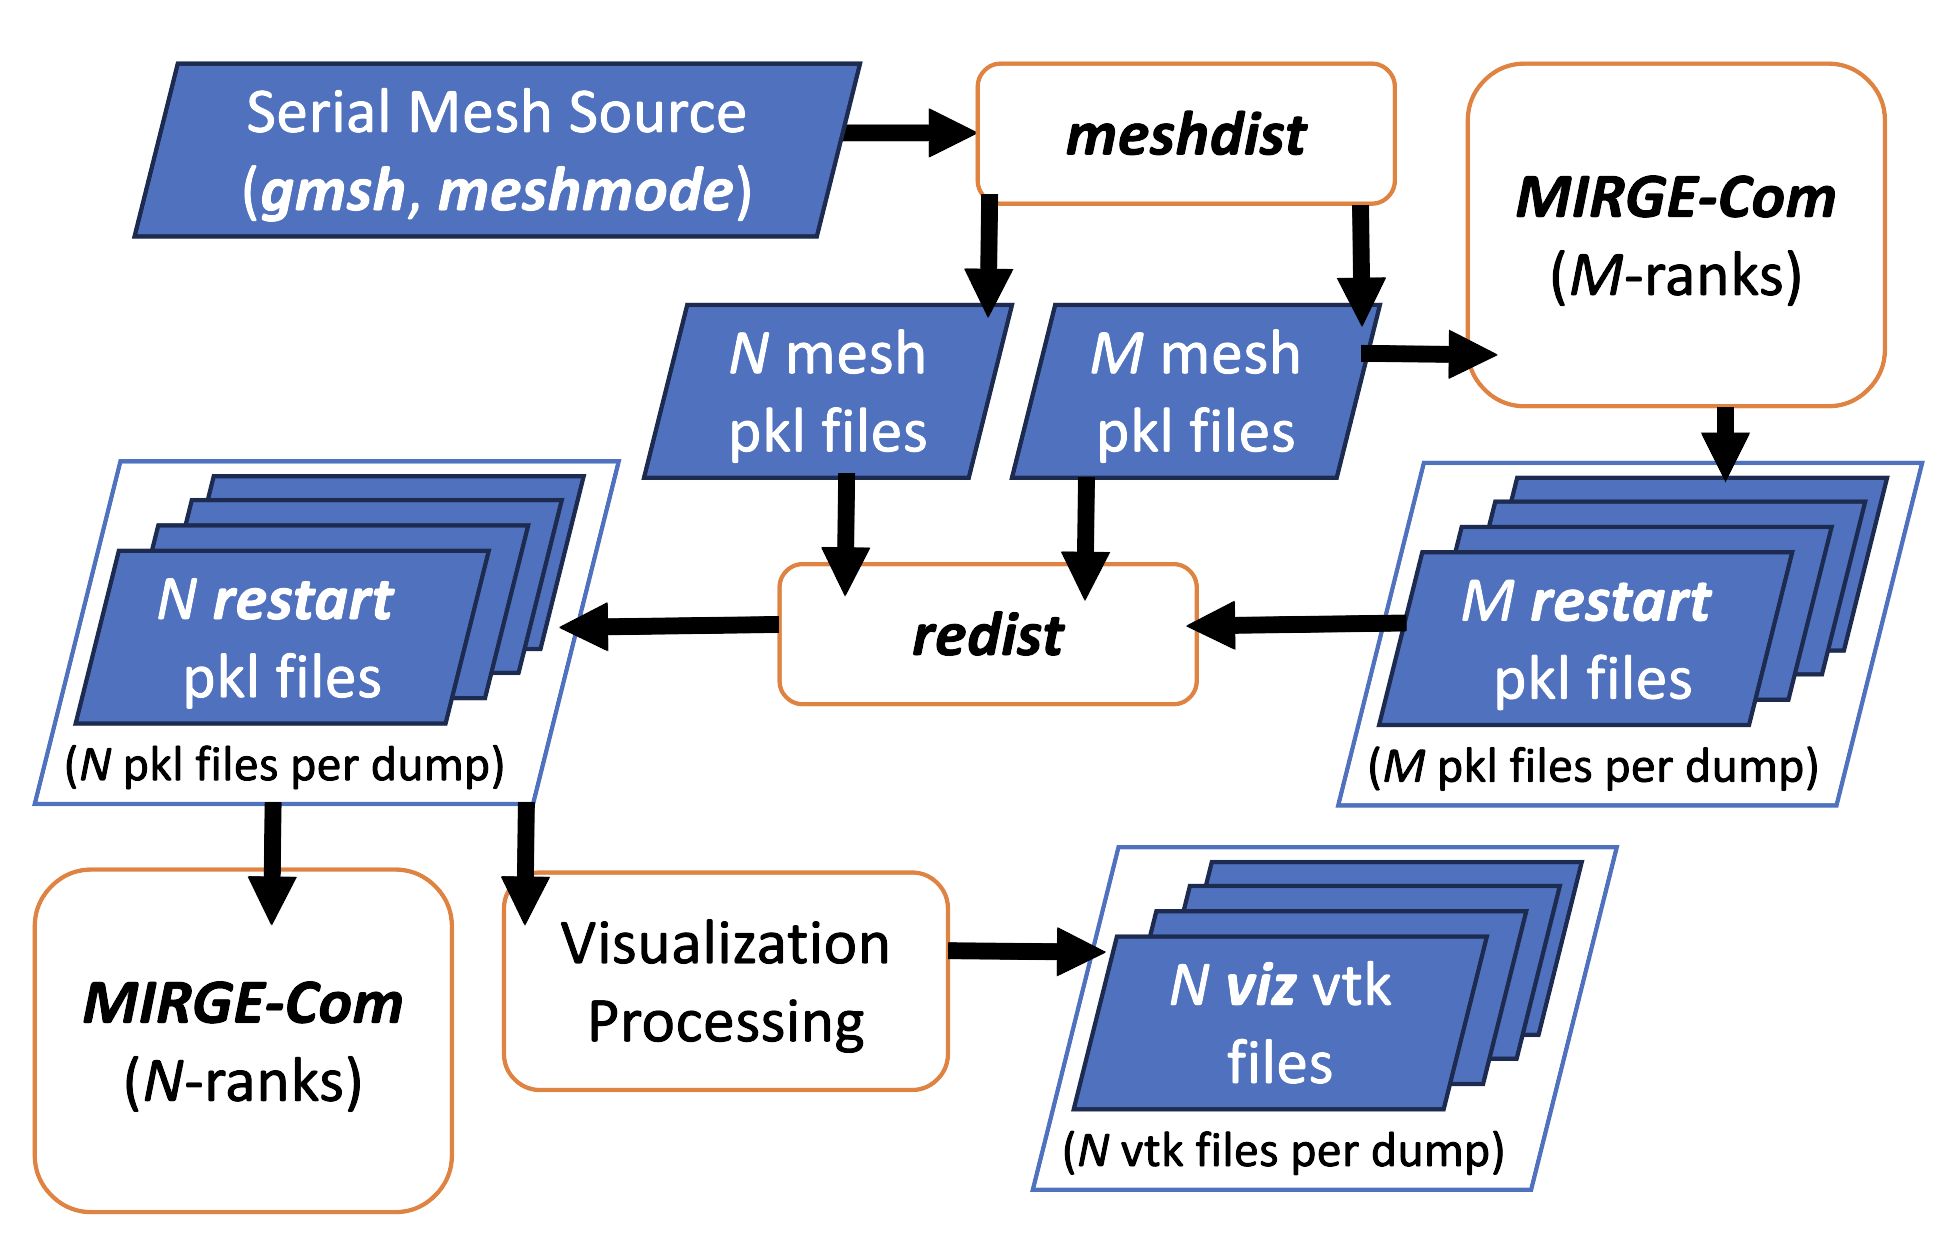
\includegraphics[width=\textwidth]{Figures/mtc/redist_data_flow_full.png}
\end{minipage}
\end{frame}

\begin{frame}\frametitle{M-to-N Procedure Outline}
\begin{minipage}{0.49\textwidth}
\begin{itemize}
\item Generate the input mesh (\textit{gmsh} or built-in \textit{meshmode})
\color{lightgray}
\item Create the target decompositions $M$,$N$
  \begin{itemize}
  \color{lightgray}
  \item Creates required mapping files
  \item Run \textit{meshdist} part to $M$, $N$ ranks
  \end{itemize}
\item Run \mirgecom{} on $M$ ranks
\begin{itemize}
\color{lightgray}
%\item Example: Reading pre-generated mesh
\item Generates $M$ restart files per dump
\end{itemize}
\item Perform M-to-N transfer with \textit{redist}
\item Restart \mirgecom{} on $N$ ranks -or-
\item Post-processing/viz for $N$ ranks
\end{itemize}
\end{minipage}
\hfill
\begin{minipage}{.49\textwidth}
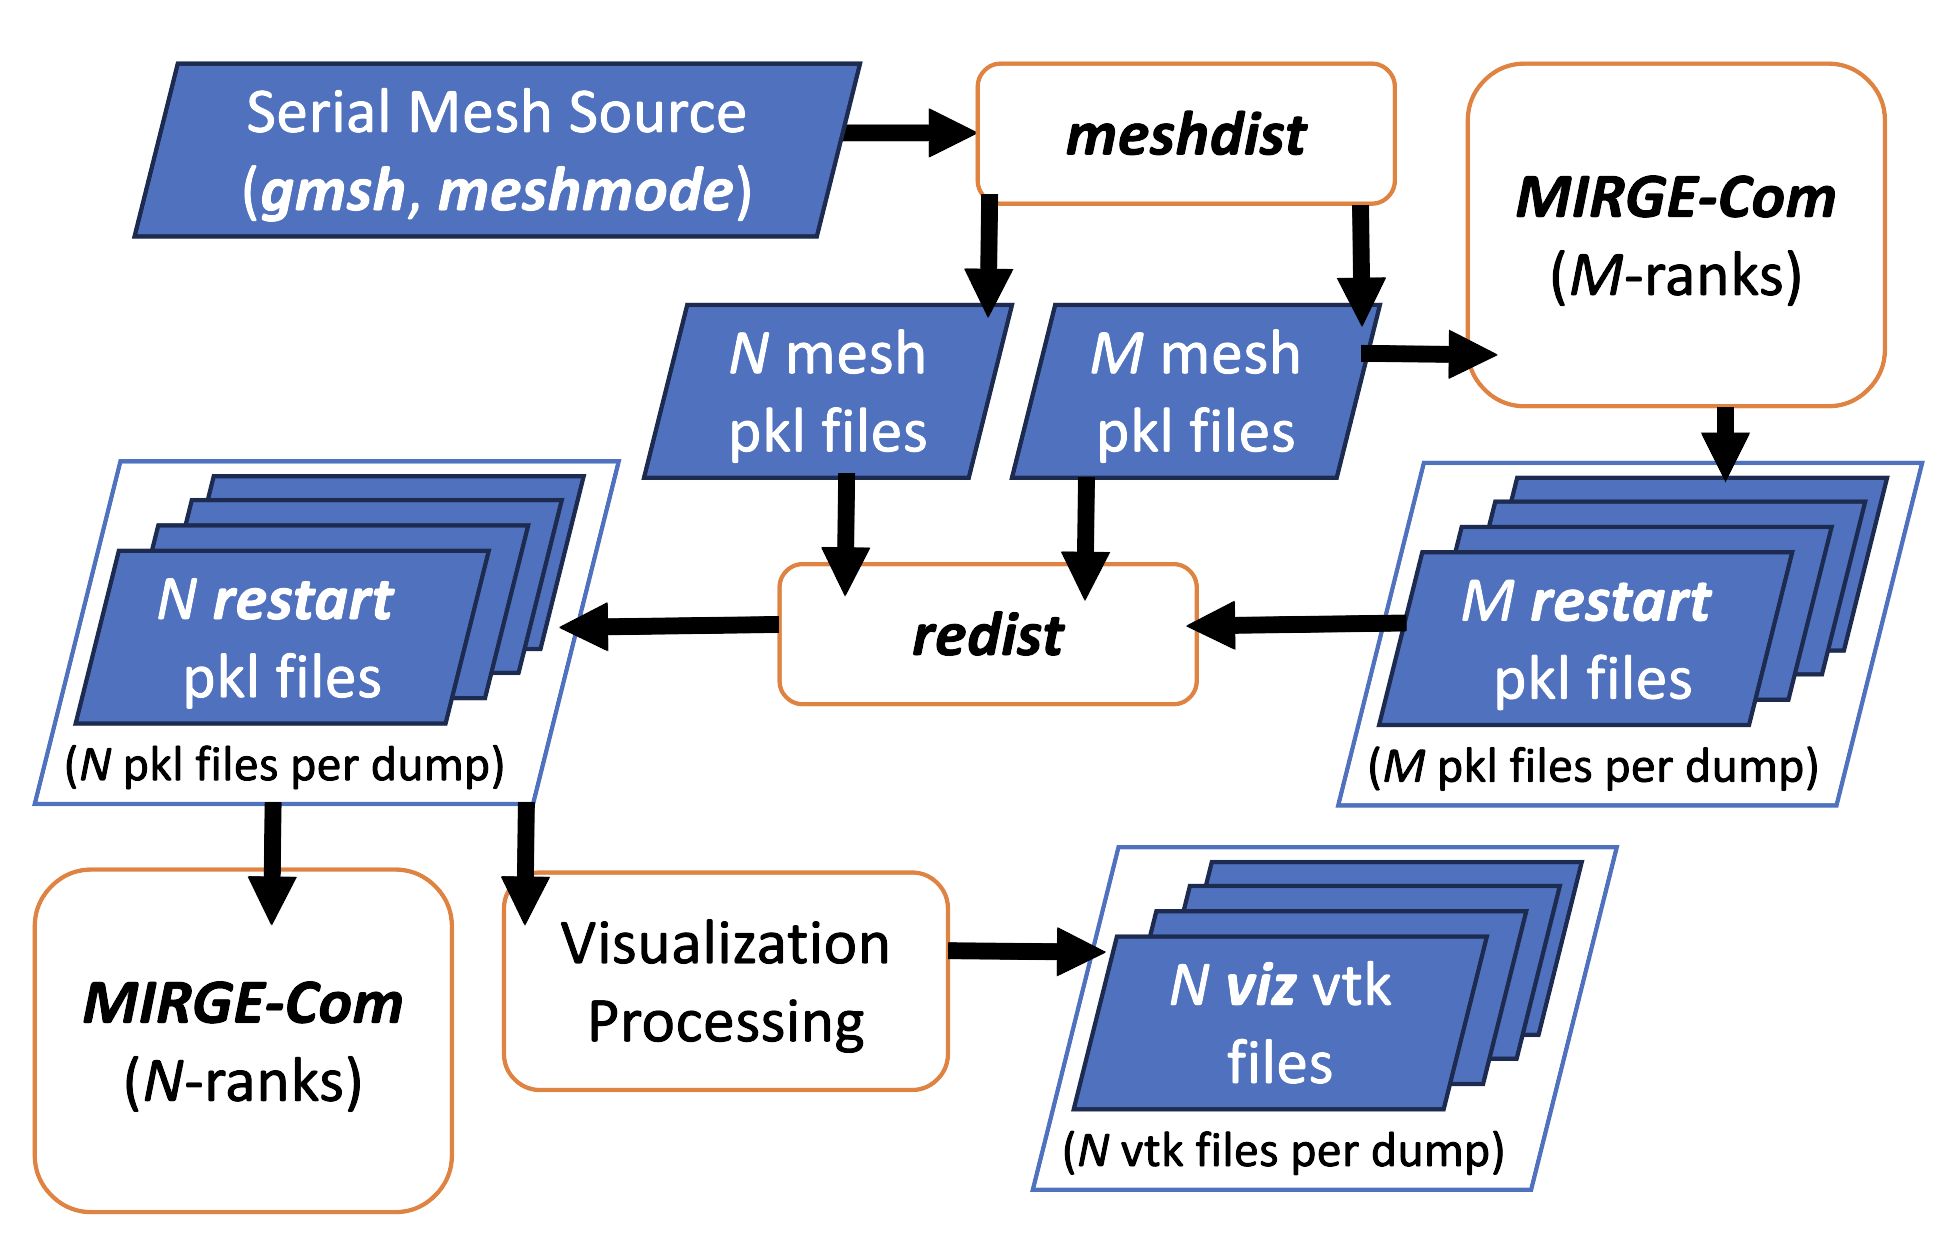
\includegraphics[width=\textwidth]{Figures/mtc/redist_data_flow_full.png}
\end{minipage}
\end{frame}


% ========= Simple examples of grid generation and import from gmsh ==============
\begin{frame}[fragile]\frametitle{Generate a Mesh with Meshmode \prj{\tiny}{M.~Smith}}

\begin{minipage}{0.5\textwidth}
\begin{itemize}
\item Mesh generator functions in \textit{meshmode} can be used to create simple
  geometries
\end{itemize}
\end{minipage}

\begin{tikzpicture}[overlay,remember picture]
\node(code)at([xshift=-1.3in,yshift=-0.5in]current page.center){
  \begin{minipage}{0.5\textwidth}
    \begin{lstlisting}[style=mintedlike,basicstyle=\mintedlikebasicstyle{\footnotesize}]
  from meshmode.mesh.generation import \
      generate_regular_rect_mesh
  mesh = generate_regular_rect_mesh(
      a=(-L/2, -L/2),
      b=(L/2, L/2),
      n=16,
      boundary_tag_to_face={
          "LeftRight": ["-x", "+x"],
          "BottomTop": ["-y", "+y"]})
    \end{lstlisting}
  \end{minipage}
};
\end{tikzpicture}
\hfill
\begin{minipage}{0.5\textwidth}

\begin{tikzpicture}[scale=0.4]
    % Grid
    \draw[step=1, thin, black] (0,0) grid (16,10);
    \draw[thick] (0,0) rectangle (16,10);
\end{tikzpicture}
\end{minipage}

\end{frame}

\begin{frame}[fragile]\frametitle{Generate Multivolume Mesh with Meshmode}

\begin{minipage}{0.5\textwidth}
\begin{itemize}
\item Creation of multi-volume mesh with \textit{meshmode}
\end{itemize}
\end{minipage}

\begin{tikzpicture}[overlay,remember picture]
\node(code)at([xshift=-1.3in,yshift=-0.5in]current page.center){
  \begin{minipage}{0.5\textwidth}
    \begin{lstlisting}[style=mintedlike,basicstyle=\mintedlikebasicstyle{\footnotesize}]
  from meshmode.mesh.generation import \
      generate_regular_rect_mesh
  mesh = generate_regular_rect_mesh(
      a=(-L/2, -L/2),
      b=(L/2, L/2),
      n=16,
      boundary_tag_to_face={
          "LeftRight": ["-x", "+x"],
          "BottomTop": ["-y", "+y"]})
  x_avg = np.sum(x, axis=1)/x.shape[1]
  tag_to_elements = {
      "Vol1": np.where(x_avg < vol1_loc)[0],
      "Vol2": np.where(x_avg > vol1_loc)[0]}
    \end{lstlisting}
  \end{minipage}
};
\end{tikzpicture}
\hfill
\begin{minipage}{0.5\textwidth}
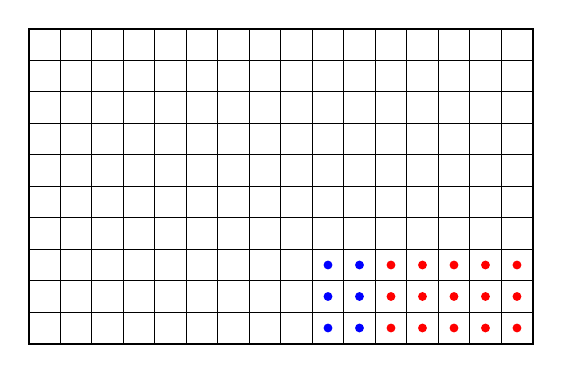
\begin{tikzpicture}[scale=0.4]
    % Grid
    \draw[step=1, thin, black] (0,0) grid (16,10);
    \draw[thick] (0,0) rectangle (16,10);
    % Red subregion
    \foreach \i in {11, 12, 13, 14, 15} {
        \foreach \j in {0, 1, 2} {
            \fill[red] (\i+0.5, \j+0.5) circle (4pt);
        }
    }
    
    % Blue subregion
    \foreach \i in {9, 10} {
        \foreach \j in {0, 1, 2} {
            \fill[blue] (\i+0.5, \j+0.5) circle (4pt);
        }
    }
\end{tikzpicture}
\begin{tikzpicture}[overlay, remember picture, scale=0.3]
  % Legend Box
  \begin{scope}[xshift=-20.8cm, yshift=16.8cm]
    \draw[thick] (-1,0.5) rectangle (6,-3);
   
    \fill[blue] (0,-0.5) circle (6pt); % Blue dot
    \node[align=left] at (3,-0.5) {Volume 1};
     
    \fill[red] (0,-2) circle (6pt);  % Red dot
    \node[align=left] at (3,-2) {Volume 2};
  \end{scope}
\end{tikzpicture}
\end{minipage}

\end{frame}


\begin{frame}[fragile]\frametitle{Generate a Tensor Product Mesh with Meshmode}

\begin{minipage}{0.5\textwidth}
\begin{itemize}
\item Creation of tensor product element mesh with \textit{meshmode}
\end{itemize}
\end{minipage}

\begin{tikzpicture}[overlay,remember picture]
\node(code)at([xshift=-1.3in,yshift=-0.5in]current page.center){
  \begin{minipage}{0.5\textwidth}
    \begin{lstlisting}[style=mintedlike,basicstyle=\mintedlikebasicstyle{\footnotesize}]
  from meshmode.mesh import \
      TensorProductElementGroup
  from meshmode.mesh.generation import \
      generate_regular_rect_mesh
  mesh = generate_regular_rect_mesh(
      a=(-L/2, -L/2),
      b=(L/2, L/2),
      n=16,
      boundary_tag_to_face={
          "LeftRight": ["-x", "+x"],
          "BottomTop": ["-y", "+y"]},
      group_cls=TensorProductElementGroup)
    \end{lstlisting}
  \end{minipage}
};
\end{tikzpicture}
\hfill
\begin{minipage}{0.5\textwidth}

\begin{tikzpicture}[scale=0.4]
    % Grid
    \draw[step=1, thin, black] (0,0) grid (16,10);
    \draw[thick] (0,0) rectangle (16,10);
\end{tikzpicture}
\end{minipage}

\end{frame}


\begin{frame}[fragile]\frametitle{Import a Gmsh Mesh \prj{\tiny}{M.~Smith}}
\vspace{-0.9in}

\begin{minipage}{0.5\textwidth}
\begin{itemize}
\item Otherwise, use \textit{Gmsh} to generate meshes from CAD
\item Multi-volume supported natively in \textit{Gmsh}
\end{itemize}
\end{minipage}

\begin{tikzpicture}[overlay,remember picture]
\node(code)at([xshift=-1.3in,yshift=-0.5in]current page.center){
  \begin{minipage}{0.5\textwidth}
    \begin{lstlisting}[style=mintedlike,basicstyle=\mintedlikebasicstyle{\footnotesize}]
def get_mesh_data():
  from meshmode.mesh.io import read_gmsh
  mesh, tag_to_elements = \
    read_gmsh(
       mesh_filename, force_ambient_dim=dim,
       return_tag_to_elements_map=True)
  volume_to_tags = {
     "fluid": ["fluid"],
     "wall":  ["wall_insert", "wall_surround"]
  }
  return mesh, tag_to_elements, volume_to_tags
  \end{lstlisting}
  \end{minipage}
};
\end{tikzpicture}

\begin{tikzpicture}[overlay,remember picture]
\node(anchor)at([xshift=1.6in]current page.center){};
\node(nozzlemesh)at([yshift=0.8in]anchor.center){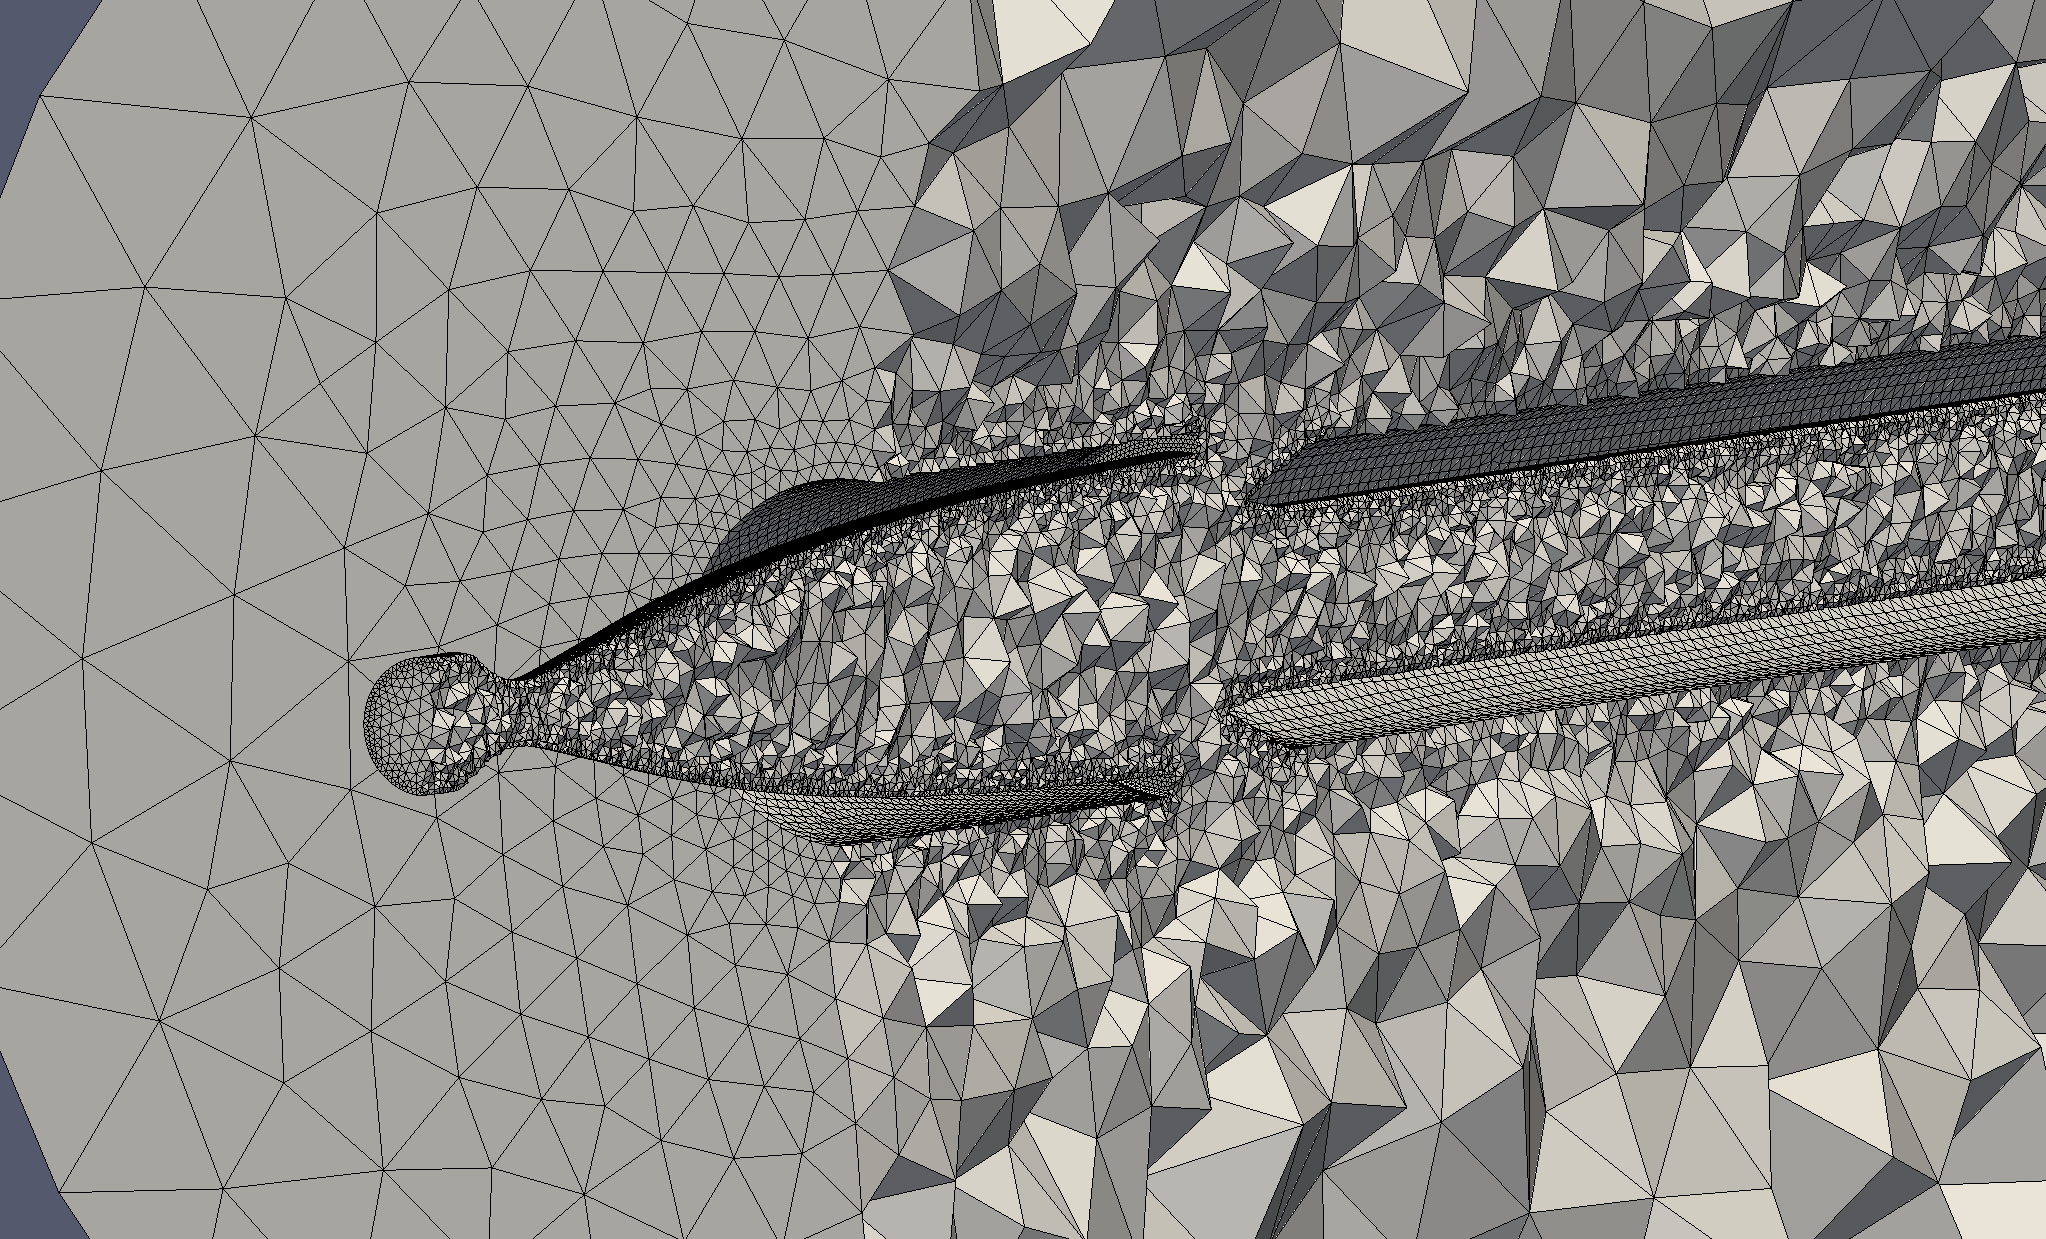
\includegraphics[width=0.4\textwidth]{Figures/mtc/nozzle_mesh.png}};
\node(y3mesh)at([yshift=-0.9in]anchor.center){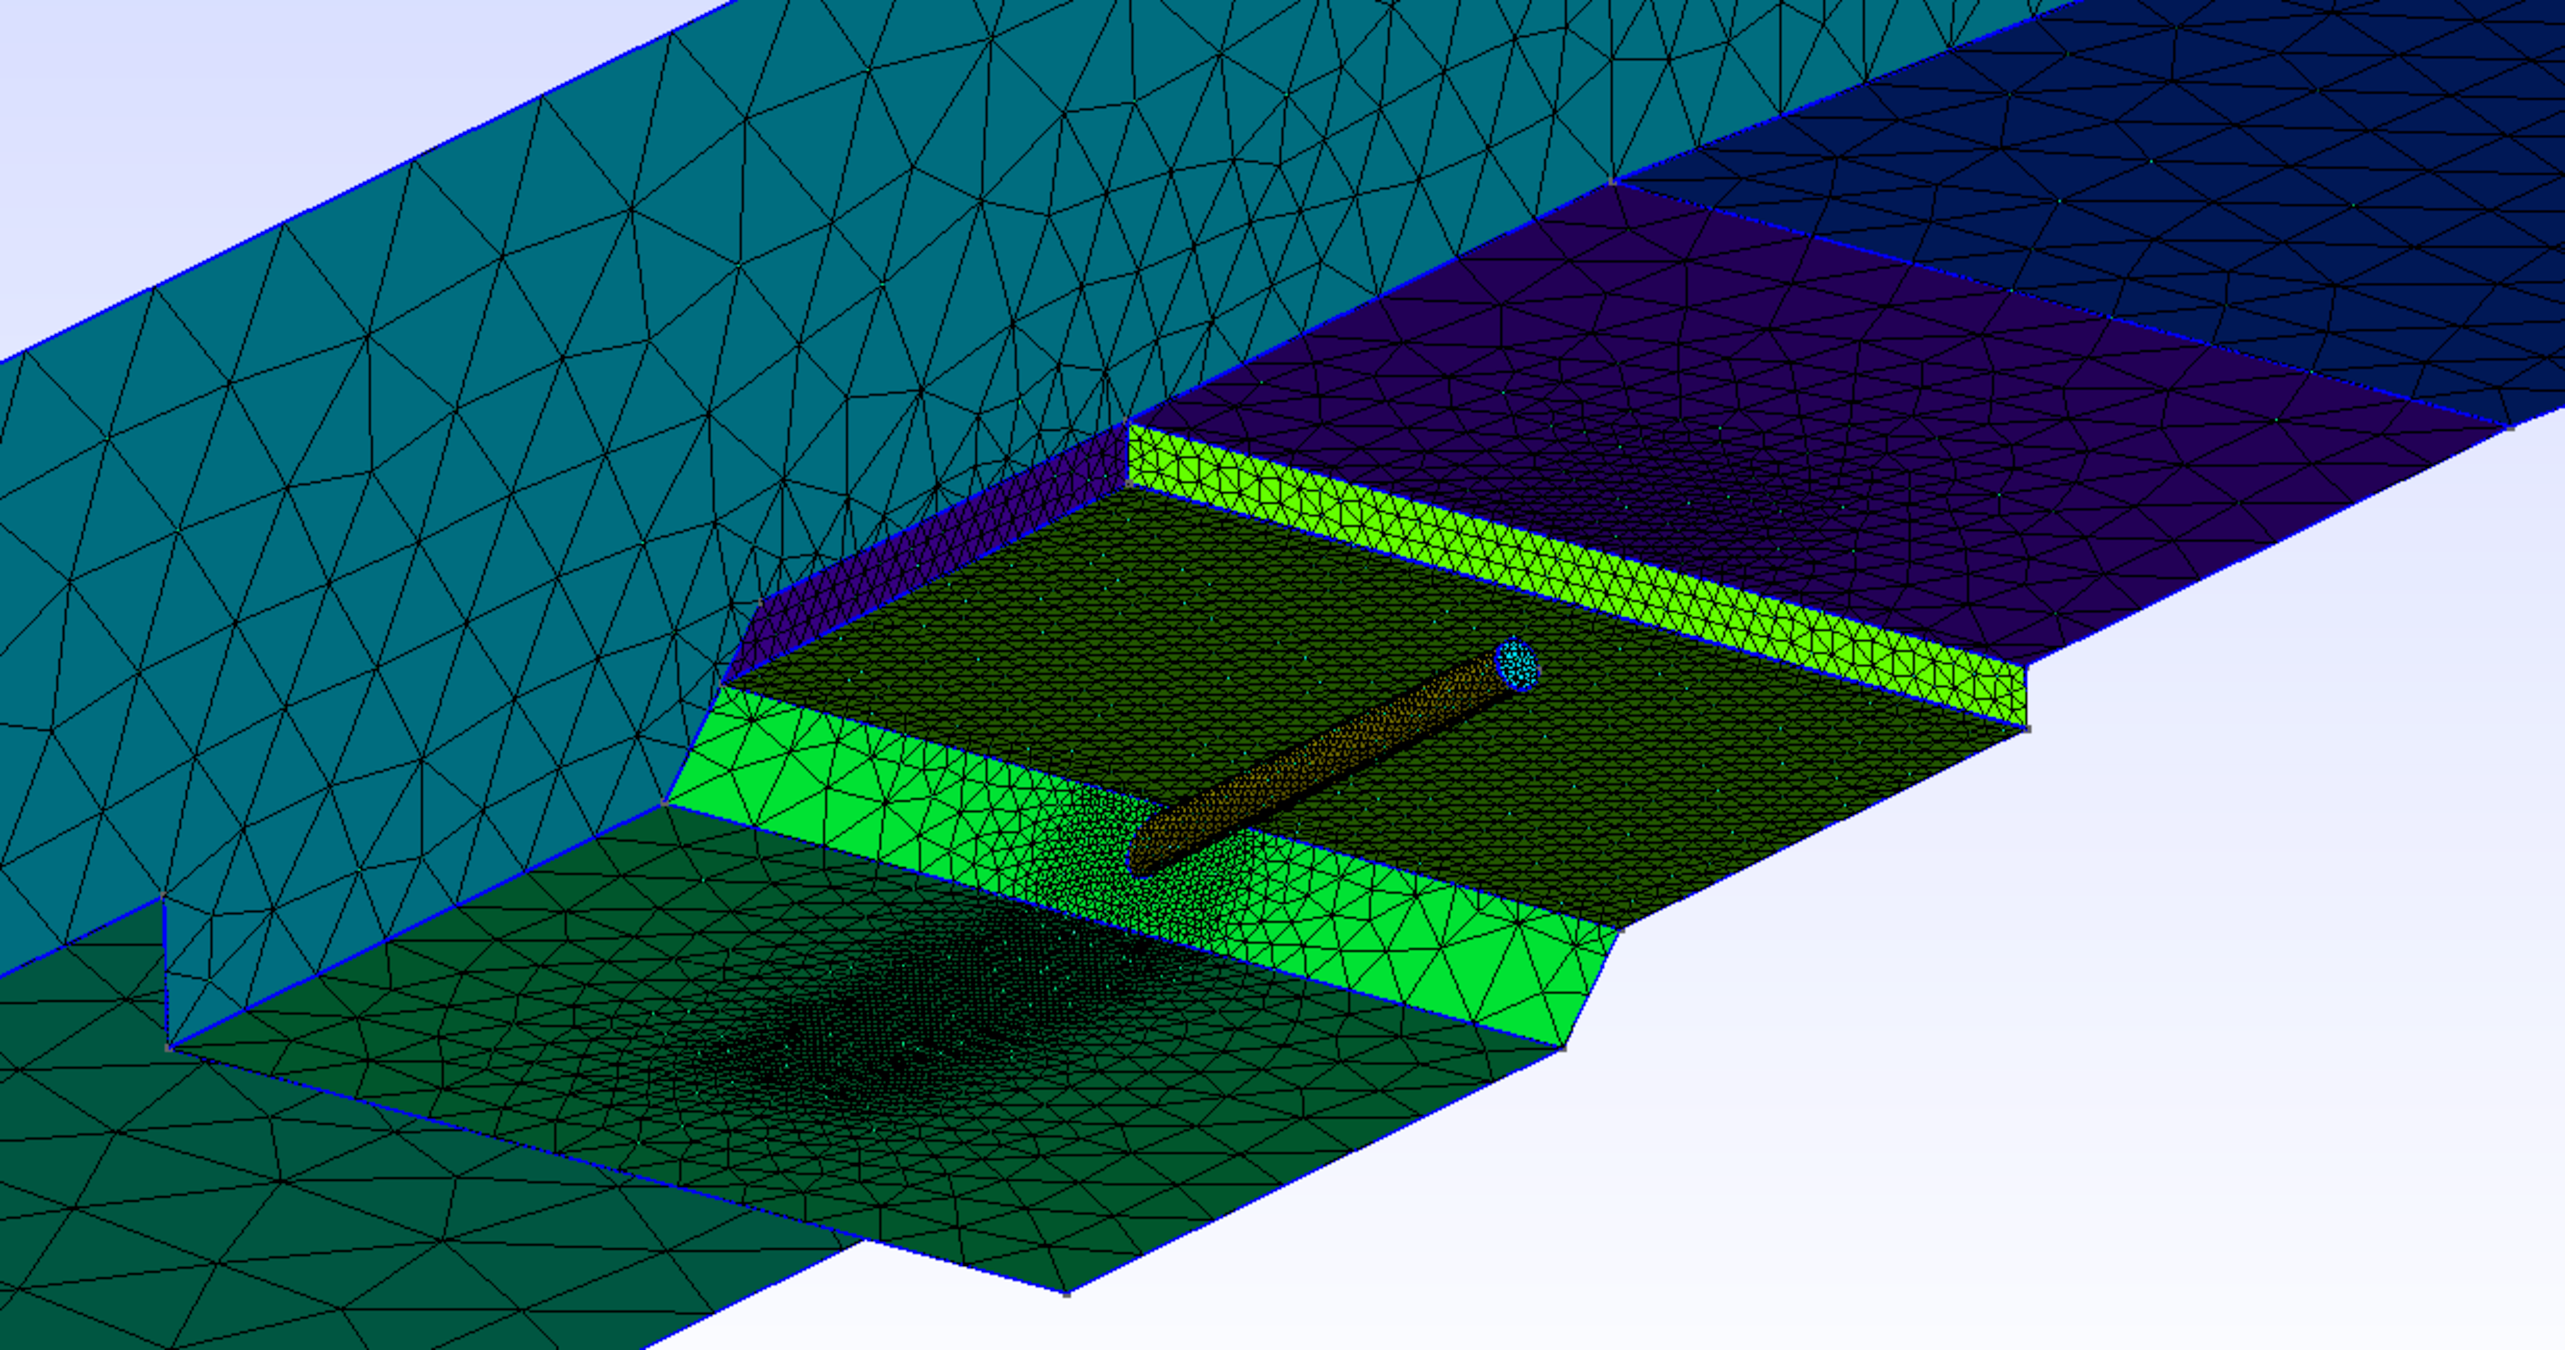
\includegraphics[width=0.4\textwidth]{Figures/mtc/3d_mesh_cavity.pdf}};
\node(ref)at([xshift=-0.1in]y3mesh.south){\prj{\tiny}{M.~Anderson, 02}};
\end{tikzpicture}

\end{frame}
% ================================================================================

% Regardless of mesh source/generator, mesh is in this general form:
\begin{frame}\frametitle{Global Mesh: Input}
\vspace{-20pt}
%\begin{minipage}[t][0.3\textheight][t]{\textwidth}
\begin{minipage}{0.5\textwidth}
\begin{itemize}
\item Gmsh, or meshmode generated mesh
  \begin{itemize}
  \item Vertex physical ($xyz$) coordinates, ($V$)
  \item Element connectivity: element-to-vertices map, ($[V][E_n]$)
  \end{itemize}
\item Total number of elements in the global mesh: $N_E$
\item Globally numbered elements: $E_n = [0, 1, 2,..., N_E)$
\item If multivolume: Tag-to-elements map, ($[E_n][tag]$)
\item Note: element numbering for unstructured mesh
\end{itemize}
\end{minipage}
\hfill
%\vfill
\begin{minipage}{0.48\textwidth}
\begin{tikzpicture}[overlay, remember picture, scale=0.4]
\begin{scope}[shift={(.5, -4)}]
    % Grid
    \draw[step=1, thin, black] (0,0) grid (16,10);
    \draw[thick] (0,0) rectangle (16,10);
    
    \def\flatteneddata{
        0, 1, 3, 6, 10, 15, 21, 28, 36, 45, 55, 65, 75, 85, 95, 105, 
        2, 4 , 7, 11, 16, 22, 29, 37, 46, 56, 66, 76, 86, 96, 106, 115, 
        5, 8, 1  2, 17, 23, 30, 38, 47, 57, 67, 77, 87, 97, 107, 116, 124, 
        9, 13, 18, 24, 31, 39, 48, 58, 68, 78, 88, 98, 108, 117, 125, 132, 
        14, 19, 25, 32, 40, 49, 59, 69, 79, 89, 99, 109, 118, 126, 133, 139, 
        20, 26, 33, 41, 50, 60, 70, 80, 90, 100, 110, 119, 127, 134, 140, 145, 
        27, 34, 42, 51, 61, 71, 81, 91, 101, 111, 120, 128, 135, 141, 146, 150, 
        35, 43, 52, 62, 72, 82, 92, 102, 112, 121, 129, 136, 142, 147, 151, 154, 
        44, 53, 63, 73, 83, 93, 103, 113, 122, 130, 137, 143, 148, 152, 155, 157, 
        54, 64, 74, 84, 94, 104, 114, 123, 131, 138, 144, 149, 153, 156, 158, 159
    }
    
    \xdef\mycount{0}
    \foreach \value in \flatteneddata {
        % Calculate x and y coordinates based on the mycount
        \pgfmathtruncatemacro\x{\mycount - 16 * (int(\mycount/16))}
        \pgfmathtruncatemacro\y{int(\mycount/16)}
        
        \node at (\x+0.5, 9.5-\y) {\tiny \value};
        
        \pgfmathtruncatemacro\incrementedcount{\mycount + 1}
        \xdef\mycount{\incrementedcount}
    }
\end{scope}
\end{tikzpicture}
\end{minipage}
\end{frame}


\begin{frame}\frametitle{M-to-N Procedure Outline}
\begin{minipage}{0.49\textwidth}
\begin{itemize}
\item {\color{lightgray}{Generate the input mesh (\textit{gmsh} or built-in \textit{meshmode}})}
\item Create the target decompositions $M$,$N$
  \begin{itemize}
  \item Creates required mapping files
  \item Run \textit{meshdist} part to $M$, $N$ ranks
  \end{itemize}
\color{lightgray}
\item Run \mirgecom{} on $M$ ranks
\begin{itemize}
\color{lightgray}
%\item Example: Reading pre-generated mesh
\item Generates $M$ restart files per dump
\end{itemize}
\item Perform M-to-N transfer with \textit{redist}
\item Restart \mirgecom{} on $N$ ranks -or-
\item Post-processing/viz for $N$ ranks
\end{itemize}
\end{minipage}
\hfill
\begin{minipage}{.49\textwidth}
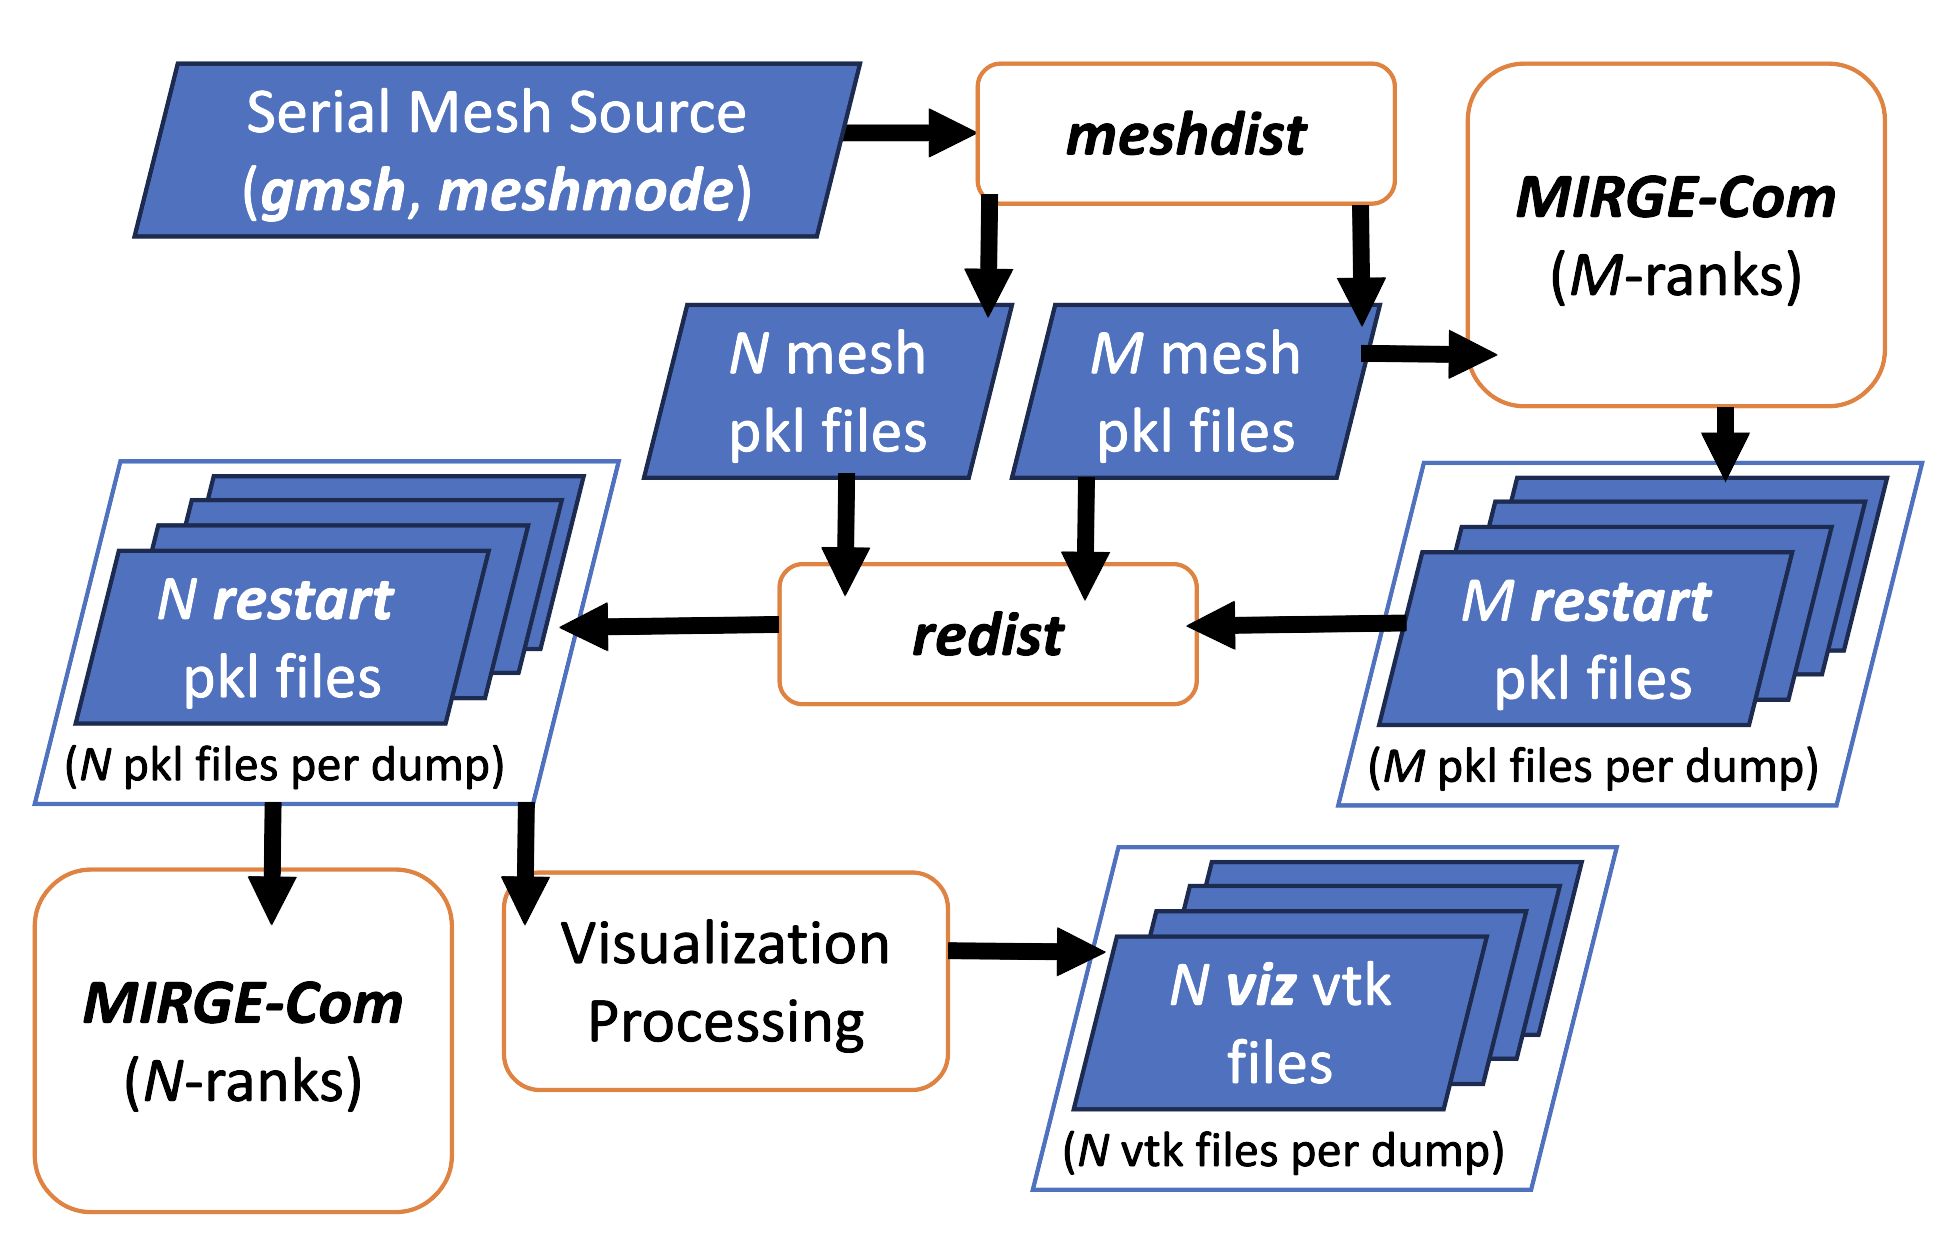
\includegraphics[width=\textwidth]{Figures/mtc/redist_data_flow_full.png}
\end{minipage}
\end{frame}

\begin{frame}\frametitle{\textit{meshdist}: \mirgecom{} Mesh Partitioning Utility}
  \begin{minipage}[t][.4\textheight][t]{\textwidth}
    \begin{multicols}{2}
      \begin{itemize}
      \item Creates $M$-decomposition of input mesh
      \item \textit{Metis} by default, 1dpart optional
      \item Mirrors built-in decomposition, \textbf{\textit{except}}:
        %\begin{itemize}
        %\item Writes mapping files required by m-to-n
          \begin{itemize}
          \item Writes decomp map: $r_m[E_N]$  (maps global element id $E_n$ to MPI rank $r_m$)
          %\item PartID map: $P[E_N]$ (maps global element id to PartID $P$)
          %\item PartID is (volume, rank) pair
          \item Writes $M$-decomposed mesh into pkl file per rank
          \end{itemize}
        %\end{itemize}
      \item Divides work across $P$ processors (max used $= M$)
        \begin{itemize}
        \item Each \textit{meshdist} rank locally handles $M/P$ mesh partitions
        \item Reads and partition input mesh on all ranks
        % \item Local meshmode datastructures for locally-handled $M$-parts
        \item Writes only locally-handled $M$-parts to pkl
        \end{itemize}
      \end{itemize}
    \end{multicols}
  \end{minipage}
  \vfill
  \center{\texttt{python -m mpi4py meshdist.py -1 -n 4 -i box.msh -o box\_4p}}
  \begin{minipage}[b][.4\textheight][t]{\textwidth}
    \begin{tikzpicture}[overlay, remember picture, scale=0.3]
      \node at (2cm, -14.5cm) (center) {};

      %\begin{scope}[shift={(center)}]  % yshift=-10cm]
      \begin{scope}[yshift=-12cm]

        % Grid
        \draw[step=1, thin, black] (0,0) grid (16,10);
        \draw[thick] (0,0) rectangle (16,10);

        \begin{scope}[xshift=30cm]
          % Partition 0
          \draw[step=1, thin, black] (0,0) grid (4,10);
          \draw[thick] (0,0) rectangle (4,10);
          \node[font=\bfseries, blue] at (2,9) {0};
    
          % Partition 1
          \begin{scope}[xshift=4.5cm]
            \draw[step=1, thin, black] (0,0) grid (4,10);
            \draw[thick] (0,0) rectangle (4,10);
            \node[font=\bfseries, blue] at (2,9) {1};
          \end{scope}
    
          % Partition 2 
          \begin{scope}[xshift=9cm]
            \draw[step=1, thin, black] (0,0) grid (4,10);
            \draw[thick] (0,0) rectangle (4,10);
            \node[font=\bfseries, blue] at (2,9) {2};
          \end{scope}
    
          % Partition 3 
          \begin{scope}[xshift=13.5cm]
            \draw[step=1, thin, black] (0,0) grid (4,10);
            \draw[thick] (0,0) rectangle (4,10);
            \node[font=\bfseries, blue] at (2,9) {3};
          \end{scope}
        \end{scope}
    
        % Coordinates for arrow
        \coordinate (leftGridCenter) at (8,5);
        \coordinate (rightGridCenter) at (38,5);
    
        % Arrow with text
        \draw[->, ultra thick] (leftGridCenter) -- node[midway, fill=white, text width=3cm, align=center] {\textit{meshdist}} (rightGridCenter);
      \end{scope}
    \end{tikzpicture}
  \end{minipage}
\end{frame}


\begin{frame}\frametitle{Multivolume Mesh with \textit{meshdist}}
  \begin{minipage}[t][.2\textheight][t]{\textwidth}
    %\begin{multicols}{2}
      \begin{itemize}
      %\item Creates $M$-decomposition of multivolume input mesh
      \item Additional data for multivolume meshes: 
          \begin{itemize}
          \item Writes PartID map: $P[E_N]$ (maps global element id to PartID $P$)
          \item PartID is (volume, rank) pair
          \end{itemize}
        %\end{itemize}
      %\item Divides work across $P$ processors (max used $= M$)
        %\begin{itemize}
        %\item Each \textit{meshdist} rank locally handles $M/P$ mesh partitions
        %\item Reads and partition input mesh on all ranks
        % \item Local meshmode datastructures for locally-handled $M$-parts
        %\item Writes only locally-handled $M$-parts to pkl
        %\end{itemize}
      \end{itemize}
    %\end{multicols}
  \end{minipage}
  \vfill
  \center{\texttt{mpiexec -n NP python -m mpi4py meshdist.py -w -1 -n 4 -i multivol.msh -o multivol\_4p}}
  \begin{minipage}[b][.4\textheight][t]{\textwidth}
    \begin{tikzpicture}[overlay, remember picture, scale=0.3]
      \begin{scope}[yshift=-12cm]
        % Grid
        \draw[step=1, thin, black] (0,0) grid (16,10);
        \draw[thick] (0,0) rectangle (16,10);
    
        % Red subregion
        \foreach \i in {11, 12, 13, 14, 15} {
          \foreach \j in {0, 1, 2} {
            \fill[red] (\i+0.5, \j+0.5) circle (4pt);
          }
        }
    
        % Blue subregion
        \foreach \i in {9, 10} {
          \foreach \j in {0, 1, 2} {
            \fill[blue] (\i+0.5, \j+0.5) circle (4pt);
          }
        }
        \begin{scope}[xshift=30cm]
          % Partition 0
          \draw[step=1, thin, black] (0,0) grid (4,10);
          \draw[thick] (0,0) rectangle (4,10);
          \node[font=\bfseries, blue] at (2,9) {0};
    
          % Partition 1
          \begin{scope}[xshift=4.5cm]
            \draw[step=1, thin, black] (0,0) grid (4,10);
            \draw[thick] (0,0) rectangle (4,10);
            \node[font=\bfseries, blue] at (2,9) {1};
          \end{scope}
    
          % Partition 2 with blue and red subregions
          \begin{scope}[xshift=9cm]
            \draw[step=1, thin, black] (0,0) grid (4,10);
            \draw[thick] (0,0) rectangle (4,10);
            \foreach \j in {0, 1, 2} {
              \fill[blue] (1.5, \j+0.5) circle (4pt);
              \fill[blue] (2.5, \j+0.5) circle (4pt);
              \fill[red] (3.5, \j+0.5) circle (4pt);
            }
            \node[font=\bfseries, blue] at (2,9) {2};
          \end{scope}
    
          % Partition 3 with red subregion
          \begin{scope}[xshift=13.5cm]
            \draw[step=1, thin, black] (0,0) grid (4,10);
            \draw[thick] (0,0) rectangle (4,10);
            \foreach \j in {0, 1, 2} {
              \fill[red] (0.5, \j+0.5) circle (4pt);
              \fill[red] (1.5, \j+0.5) circle (4pt);
              \fill[red] (2.5, \j+0.5) circle (4pt);
              \fill[red] (3.5, \j+0.5) circle (4pt);
            }
            \node[font=\bfseries, blue] at (2,9) {3};
          \end{scope}
        \end{scope}
        % Coordinates for arrow
        \coordinate (leftGridCenter) at (8,5);
        \coordinate (rightGridCenter) at (38,5);
        
        % Arrow with text
        \draw[->, ultra thick] (leftGridCenter) -- node[midway, fill=white, text width=3cm, align=center] {\textit{meshdist}} (rightGridCenter);
      \end{scope}
    \end{tikzpicture}
  \end{minipage}
\end{frame}

\begin{frame}\frametitle{M-to-N Procedure Outline}
\begin{minipage}{0.49\textwidth}
\begin{itemize}
\item {\color{lightgray}{Generate the input mesh (\textit{gmsh} or built-in \textit{meshmode}})}
\item {\color{lightgray}{Create the target decompositions $M$,$N$}}
  \begin{itemize}
  \color{lightgray}
  \item Creates required mapping files
  \item Run \textit{meshdist} part to $M$, $N$ ranks
  \end{itemize}
\item Run \mirgecom{} on $M$ ranks
\begin{itemize}
%\item Example: Reading pre-generated mesh
\item Generates $M$ restart files per dump
\end{itemize}
\color{lightgray}
\item Perform M-to-N transfer with \textit{redist}
\item Restart \mirgecom{} on $N$ ranks -or-
\item Post-processing/viz for $N$ ranks
\end{itemize}
\end{minipage}
\hfill
\begin{minipage}{.49\textwidth}
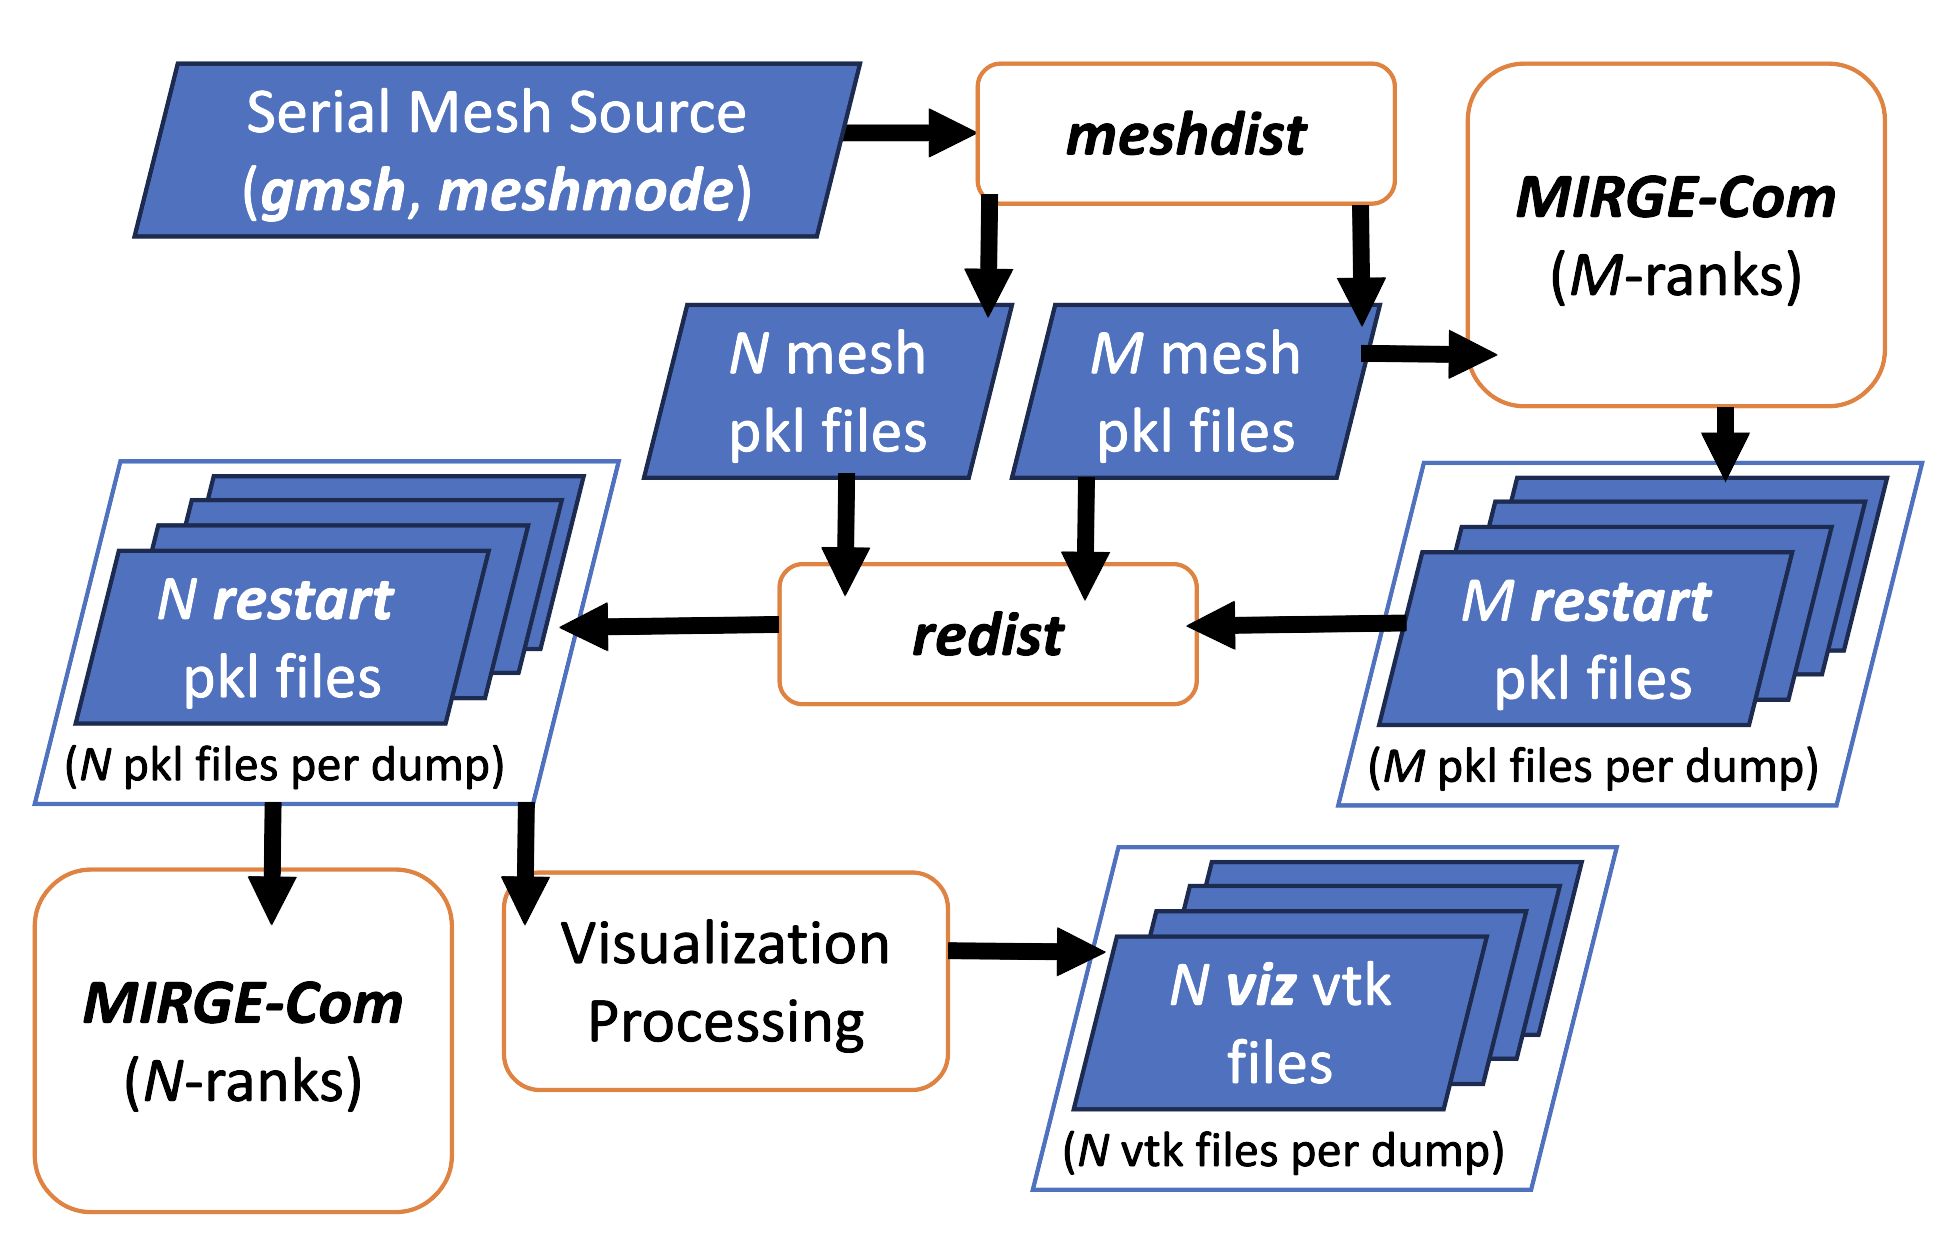
\includegraphics[width=\textwidth]{Figures/mtc/redist_data_flow_full.png}
\end{minipage}
\end{frame}

\begin{frame}\frametitle{Run \mirgecom{} on $M$ MPI Ranks (Multivolume)}
   \begin{minipage}[t][.4\textheight][t]{\textwidth}
    %\begin{multicols}{2}
      \begin{itemize}
      \item Reads $M$-partitioned input mesh
      \item Initializes \textit{volume-specific} solution
      \item Each solution dump is 1 PKL file per MPI rank with:
        \begin{itemize}
        \item Volume-specific DOFArray sizes correspond to PartIDs
        \item Arbitrary data structures in I/O dictionary 
        \end{itemize}
      \end{itemize}
    %\end{multicols}
  \end{minipage}
  \vfill
  \center{\texttt{mpiexec -n 4 python -m mpi4py prediction.py -i run\_params.yaml --lazy}}
  \begin{minipage}[b][.4\textheight][t]{\textwidth}
    \begin{tikzpicture}[overlay, remember picture, scale=0.25]
      \node at (2cm, -14.5cm) (center) {};

      %\begin{scope}[shift={(center)}]  % yshift=-10cm]
      \begin{scope}[yshift=-12cm]
        % Partition 0
        \draw[step=1, thin, black] (0,0) grid (4,10);
        \draw[thick] (0,0) rectangle (4,10);
        \node[font=\bfseries, blue] at (2,9) {0};
        
        % Partition 1
        \begin{scope}[xshift=4.5cm]
          \draw[step=1, thin, black] (0,0) grid (4,10);
          \draw[thick] (0,0) rectangle (4,10);
          \node[font=\bfseries, blue] at (2,9) {1};
        \end{scope}
    
        % Partition 2 with blue and red subregions
        \begin{scope}[xshift=9cm]
          \draw[step=1, thin, black] (0,0) grid (4,10);
          \draw[thick] (0,0) rectangle (4,10);
          \foreach \j in {0, 1, 2} {
            \fill[blue] (1.5, \j+0.5) circle (4pt);
            \fill[blue] (2.5, \j+0.5) circle (4pt);
            \fill[red] (3.5, \j+0.5) circle (4pt);
          }
          \node[font=\bfseries, blue] at (2,9) {2};
        \end{scope}
    
        % Partition 3 with red subregion
        \begin{scope}[xshift=13.5cm]
          \draw[step=1, thin, black] (0,0) grid (4,10);
          \draw[thick] (0,0) rectangle (4,10);
          \foreach \j in {0, 1, 2} {
            \fill[red] (0.5, \j+0.5) circle (4pt);
            \fill[red] (1.5, \j+0.5) circle (4pt);
            \fill[red] (2.5, \j+0.5) circle (4pt);
            \fill[red] (3.5, \j+0.5) circle (4pt);
          }
          \node[font=\bfseries, blue] at (2,9) {3};
        \end{scope}
        \begin{scope}[xshift=40cm]
          % Partition (0,0)
          \draw[step=1, thin, black] (0,0) grid (4,10);
          \draw[thick] (0,0) rectangle (4,10);
          \node[font=\bfseries, blue] at (2,9) {(0,0)};

          % Partition (1,0)
          \begin{scope}[xshift=4.5cm]
            \draw[step=1, thin, black] (0,0) grid (4,10);
            \draw[thick] (0,0) rectangle (4,10);
            \node[font=\bfseries, blue] at (2,9) {(1,0)};
          \end{scope}

          % Partition (2,0) 
          \begin{scope}[xshift=9cm]
            \foreach \i in {0,1,2,3} {
              \foreach \j in {3,4,...,9} {
                \draw (\i,\j) rectangle (\i+1,\j+1);
              }
            }
            \draw (0,0) rectangle (1,3);
            \draw (0,0) rectangle (1,1);
            \draw (0,1) rectangle (1,2);
            \draw (0,2) rectangle (1,3);
            \draw[thick] (0,0) -- (1,0) -- (1,3) -- (4,3) -- (4,10) -- (0,10) -- cycle;
            \node[font=\bfseries, blue] at (2,9) {(2,0)};
          \end{scope}

          % Partition (2,1) with blue subregion
          \begin{scope}[xshift=13.5cm, yshift=6cm]
            \draw[step=1, thin, black] (0,0) grid (2,4);
            \draw[thick] (0,0) rectangle (2,4);
            \foreach \j in {0,1,2,3} {
              \fill[blue] (0.5, \j+0.5) circle (4pt);
              \fill[blue] (1.5, \j+0.5) circle (4pt);
            }
            \node[font=\bfseries, blue] at (1,3) {(2,1)};
          \end{scope}

          % Partition (2,2) with red subregion
          \begin{scope}[xshift=13.5cm, yshift=2cm]
            \draw[step=1, thin, black] (0,0) grid (1,3);
            \draw[thick] (0,0) rectangle (1,3);
            \foreach \j in {0,1,2} {
              \fill[red] (0.5, \j+0.5) circle (4pt);
            }
            \node[font=\bfseries, blue] at (0.5,2) {(2,2)};
          \end{scope}

          % Partition (3,0)
          \begin{scope}[xshift=16cm, yshift=3.5cm]
            \draw[step=1, thin, black] (0,0) grid (4,7);
            \draw[thick] (0,0) rectangle (4,7);
            \node[font=\bfseries, blue] at (2,6) {(3,0)};
          \end{scope}

          % Partition (3,2) with red subregion
          \begin{scope}[xshift=16cm, yshift=-0.5cm]
            \draw[step=1, thin, black] (0,0) grid (4,3);
            \draw[thick] (0,0) rectangle (4,3);
            \foreach \j in {0,1,2} {
              \fill[red] (0.5, \j+0.5) circle (4pt);
              \fill[red] (1.5, \j+0.5) circle (4pt);
              \fill[red] (2.5, \j+0.5) circle (4pt);
              \fill[red] (3.5, \j+0.5) circle (4pt);
            }
            \node[font=\bfseries, blue] at (2,2) {(3,2)};
          \end{scope}
        \end{scope}
        \begin{scope}[xshift=5cm]
          % Coordinates for arrow
          \coordinate (leftGridCenter) at (8,5);
          \coordinate (rightGridCenter) at (38,5);
        
          % Arrow with text
          \draw[->, ultra thick] (leftGridCenter) -- node[midway, fill=white, text width=3cm, align=center] {\textit{MIRGE-Com}} (rightGridCenter);
        \end{scope}
      \end{scope}
    \end{tikzpicture}
  \end{minipage}
\end{frame}

\begin{frame}\frametitle{\mirgecom{} I/O Datastructure}
  \begin{itemize}
  \item Arbitrary, user-defined I/O data from \mirgecom{}
  \item No reliable way to associate DOFArrays with PartIDs
  \item Really convenient; almost completely bonkers
  \end{itemize}
\begin{tikzpicture}
  \node at (0,0) {\snippetboxbigtab{Figures/mtc/write_restart.py}{\href{https://github.com/illinois-ceesd/drivers_y3-prediction/blob/main/y3prediction/prediction.py}{prediction\_write\_restart}}};
\end{tikzpicture}
\end{frame}

\begin{frame}\frametitle{M-to-N Procedure Outline}
\begin{minipage}{0.49\textwidth}
\begin{itemize}
\item {\color{lightgray}{Generate the input mesh (\textit{gmsh} or built-in \textit{meshmode}})}
\item {\color{lightgray}{Create the target decompositions $M$,$N$}}
  \begin{itemize}
  \color{lightgray}
  \item Creates required mapping files
  \item Run \textit{meshdist} part to $M$, $N$ ranks
  \end{itemize}
\item {\color{lightgray}{Run \mirgecom{} on $M$ ranks}}
  \begin{itemize}
    \color{lightgray}
    %\item Example: Reading pre-generated mesh
  \item Generates $M$ restart files per dump
  \end{itemize}
\item Perform M-to-N transfer with \textit{redist}
\color{lightgray}
\item Restart \mirgecom{} on $N$ ranks -or-
\item Post-processing/viz for $N$ ranks
\end{itemize}
\end{minipage}
\hfill
\begin{minipage}{.49\textwidth}
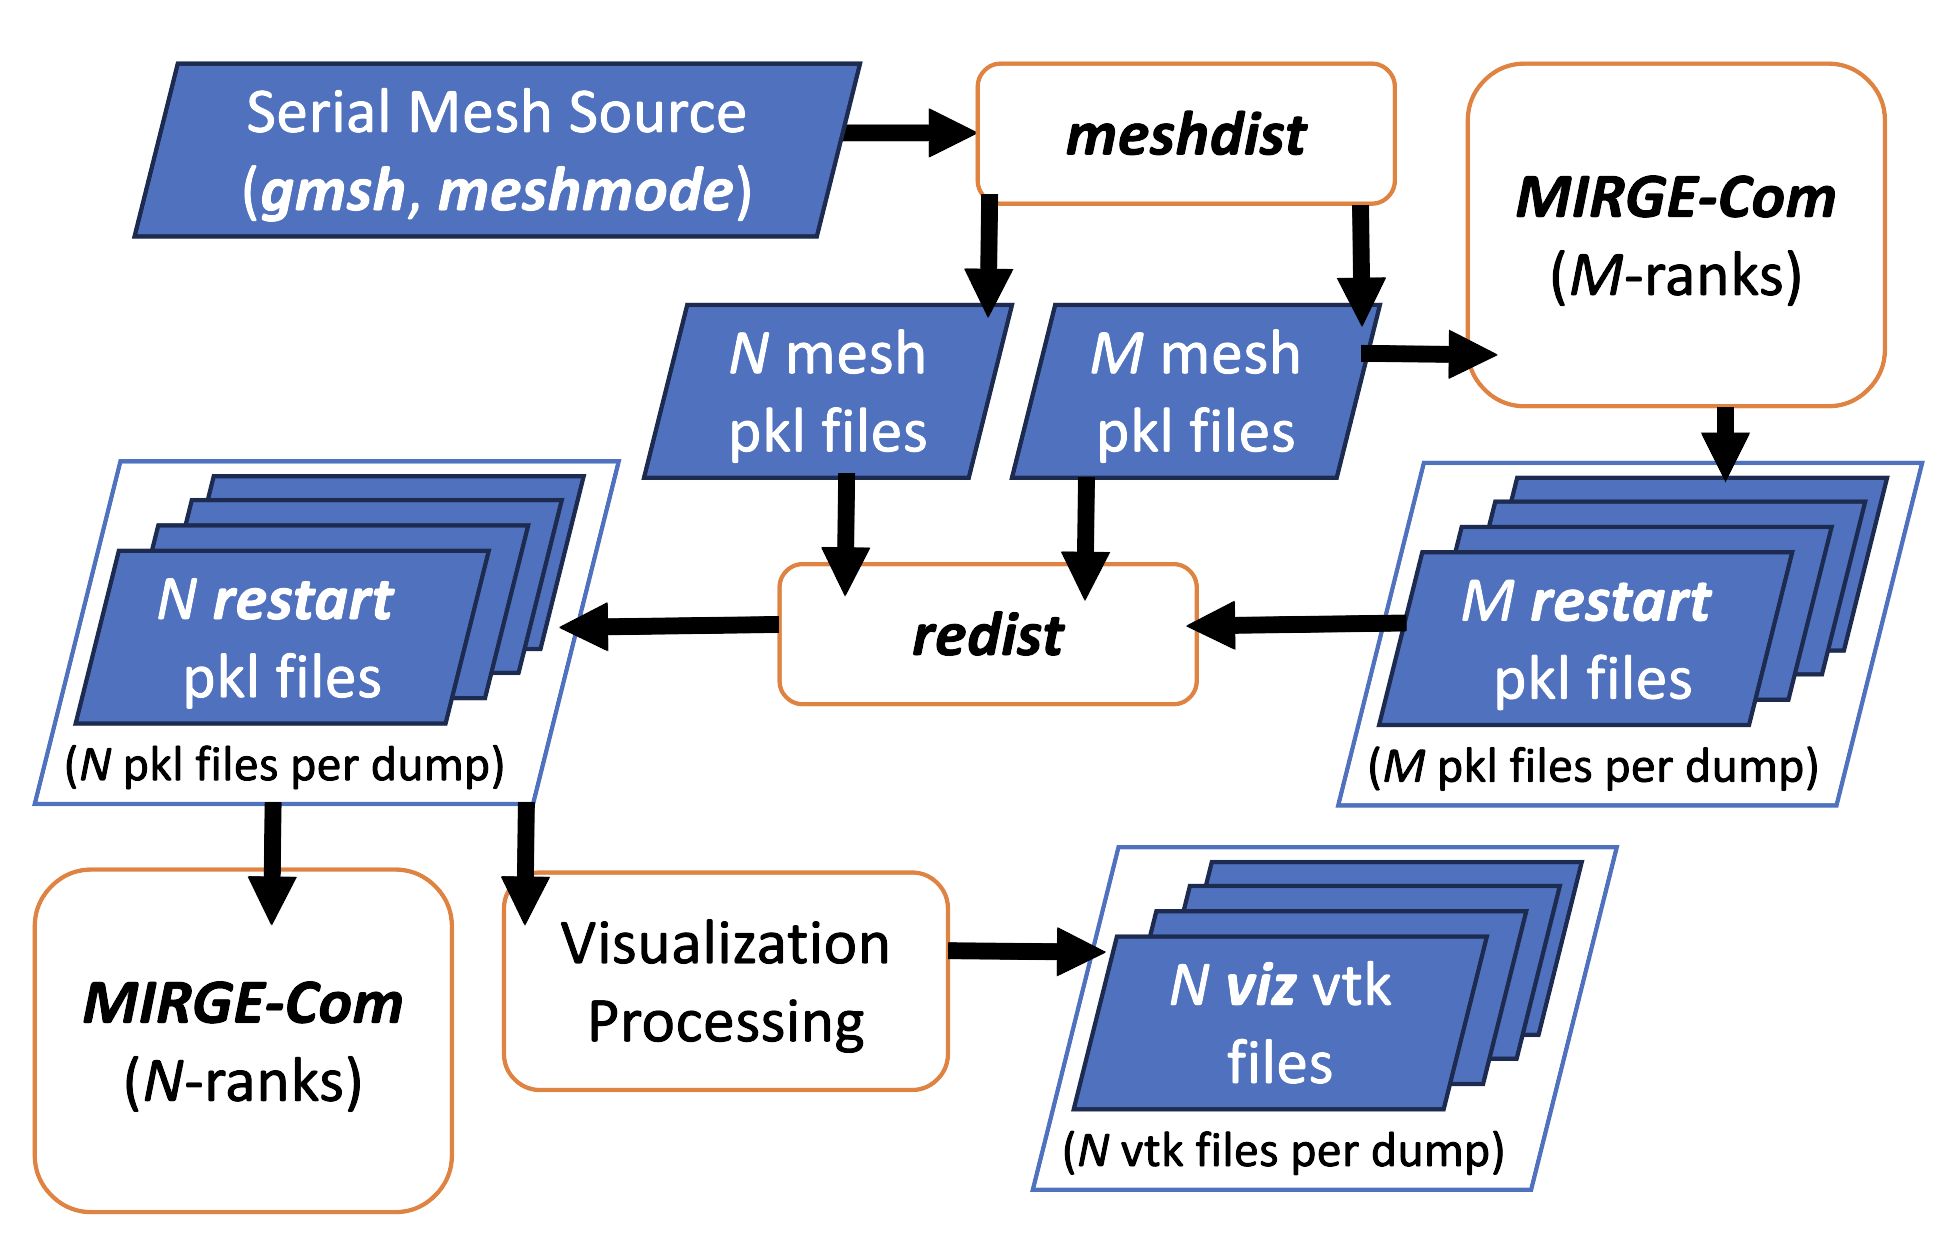
\includegraphics[width=\textwidth]{Figures/mtc/redist_data_flow_full.png}
\end{minipage}
\end{frame}

\begin{frame}\frametitle{M-to-N Transfer with \textit{redist}}
  \begin{minipage}[t][.4\textheight][t]{\textwidth}
    \begin{multicols}{2}
      \begin{itemize}
      \item Input: $M$-data (\mirgecom{} restart pkl files), $M$-decomp, $N$-decomp
      \item Unbonks the restart data with kludges:
        \begin{itemize}
        \item Detect DOFArrays in restart data: Must find an $M$-partition with \textit{all} volumes
        \item Compares DOFArray sizes to $M$-part volume sizes for volume-to-DOFArray correspondence
        \end{itemize}
      \item Creates DOFArray index mapping: $M$-decomp-local $\rightarrow$ $N$-decomp-local
      \item Reads and copies necessary $M$-data pkl files to cover $N$-part elements
      \item Writes $N$-data (new \mirgecom{} restart pkl files)
      \item Runs on arbitrary resource, dividing work like \textit{meshdist} 
      \end{itemize}
    \end{multicols}
  \end{minipage}
  \vfill
  \center{\texttt{redist.py -m 4 -n 3 -i rst\_4p -s mesh\_4p -t mesh\_3p -o rst\_3p}}
  \begin{minipage}[b][.4\textheight][t]{\textwidth}
    \begin{tikzpicture}[overlay, remember picture, scale=0.25]
      \node at (2cm, -14.5cm) (center) {};

      %\begin{scope}[shift={(center)}]  % yshift=-10cm]
      \begin{scope}[yshift=-12cm]
        % Partition (0,0)
        \draw[step=1, thin, black] (0,0) grid (4,10);
        \draw[thick] (0,0) rectangle (4,10);
        \node[font=\bfseries, blue] at (2,9) {(0,0)};
        
        % Partition (1,0)
        \begin{scope}[xshift=4.5cm]
          \draw[step=1, thin, black] (0,0) grid (4,10);
          \draw[thick] (0,0) rectangle (4,10);
          \node[font=\bfseries, blue] at (2,9) {(1,0)};
        \end{scope}

        % Partition (2,0)
        \begin{scope}[xshift=9cm]
          \foreach \i in {0,1,2,3} {
            \foreach \j in {3,4,...,9} {
              \draw (\i,\j) rectangle (\i+1,\j+1);
            }
          }
          \draw (0,0) rectangle (1,3);
          \draw (0,0) rectangle (1,1);
          \draw (0,1) rectangle (1,2);
          \draw (0,2) rectangle (1,3);
          \draw[thick] (0,0) -- (1,0) -- (1,3) -- (4,3) -- (4,10) -- (0,10) -- cycle;
          \node[font=\bfseries, blue] at (2,9) {(2,0)};
        \end{scope}

        % Partition (2,1) with blue subregion
        \begin{scope}[xshift=13.5cm, yshift=6cm]
          \draw[step=1, thin, black] (0,0) grid (2,4);
          \draw[thick] (0,0) rectangle (2,4);
          \foreach \j in {0,1,2,3} {
            \fill[blue] (0.5, \j+0.5) circle (4pt);
            \fill[blue] (1.5, \j+0.5) circle (4pt);
          }
          \node[font=\bfseries, blue] at (1,3) {(2,1)};
        \end{scope}

        % Partition (2,2) with red subregion
        \begin{scope}[xshift=13.5cm, yshift=2cm]
          \draw[step=1, thin, black] (0,0) grid (1,3);
          \draw[thick] (0,0) rectangle (1,3);
          \foreach \j in {0,1,2} {
            \fill[red] (0.5, \j+0.5) circle (4pt);
          }
          \node[font=\bfseries, blue] at (0.5,2) {(2,2)};
        \end{scope}

        % Partition (3,0)
        \begin{scope}[xshift=16cm, yshift=3.5cm]
          \draw[step=1, thin, black] (0,0) grid (4,7);
          \draw[thick] (0,0) rectangle (4,7);
          \node[font=\bfseries, blue] at (2,6) {(3,0)};
        \end{scope}
        
        % Partition (3,2) with red subregion
        \begin{scope}[xshift=16cm, yshift=-0.5cm]
          \draw[step=1, thin, black] (0,0) grid (4,3);
          \draw[thick] (0,0) rectangle (4,3);
          \foreach \j in {0,1,2} {
            \fill[red] (0.5, \j+0.5) circle (4pt);
            \fill[red] (1.5, \j+0.5) circle (4pt);
            \fill[red] (2.5, \j+0.5) circle (4pt);
            \fill[red] (3.5, \j+0.5) circle (4pt);
          }
          \node[font=\bfseries, blue] at (2,2) {(3,2)};
        \end{scope}
        \begin{scope}[xshift=40cm]
          % Partition (0,0)
          \draw[step=1, thin, black] (0,0) grid (5,10);
          \draw[thick] (0,0) rectangle (5,10);
          \node[font=\bfseries, orange] at (2.5,9) {(0,0)};

          % Partition (1,0) (panhandle grid)
          \begin{scope}[xshift=5.5cm]
            \foreach \i in {0,1,2,3,4} {
              \foreach \j in {3,4,...,9} {
                \draw (\i,\j) rectangle (\i+1,\j+1);
              }
            }
            \foreach \i in {0,1,2} {
              \foreach \j in {0,1,2} {
                \draw (\i,\j) rectangle (\i+1,\j+1);
              }
            }
            \draw[thick] (0,0) -- (3,0) -- (3,3) -- (5,3) -- (5,10) -- (0,10) -- cycle;
            \node[font=\bfseries, orange] at (2.5,9) {(1,0)};
          \end{scope}

          % Partition (1,1) with blue subregion
          \begin{scope}[xshift=9cm, yshift=-0.5cm]
            \draw[step=1, thin, black] (0,0) grid (2,3);
            \draw[thick] (0,0) rectangle (2,3);
            \foreach \j in {0,1,2} {
              \fill[blue] (0.5, \j+0.5) circle (4pt);
              \fill[blue] (1.5, \j+0.5) circle (4pt);
            }
            \node[font=\bfseries, orange] at (1,2) {(1,1)};
          \end{scope}

          % Partition (2,0)
          \begin{scope}[xshift=12cm, yshift=3cm]
            \draw[step=1, thin, black] (0,0) grid (6,7);
            \draw[thick] (0,0) rectangle (6,7);
            \node[font=\bfseries, orange] at (3,6) {(2,0)};
          \end{scope}

          % Partition (2,2) with red subregion
          \begin{scope}[xshift=12cm, yshift=-0.5cm]
            \draw[step=1, thin, black] (0,0) grid (6,3);
            \draw[thick] (0,0) rectangle (6,3);
            \foreach \j in {0,1,2} {
              \fill[red] (0.5, \j+0.5) circle (4pt);
              \fill[red] (1.5, \j+0.5) circle (4pt);
              \fill[red] (2.5, \j+0.5) circle (4pt);
              \fill[red] (3.5, \j+0.5) circle (4pt);
              \fill[red] (4.5, \j+0.5) circle (4pt);
              \fill[red] (5.5, \j+0.5) circle (4pt);
            }
            \node[font=\bfseries, orange] at (3,2) {(2,2)};
          \end{scope}
        \end{scope}
        \begin{scope}[xshift=8cm]
          % Coordinates for arrow
          \coordinate (leftGridCenter) at (8,5);
          \coordinate (rightGridCenter) at (38,5);
        
          % Arrow with text
          \draw[->, ultra thick] (leftGridCenter) -- node[midway, fill=white, text width=3cm, align=center] {\textit{redist}} (rightGridCenter);
        \end{scope}
      \end{scope}
    \end{tikzpicture}
  \end{minipage}
\end{frame}

\begin{frame}\frametitle{M-to-N Procedure Outline}
\begin{minipage}{0.49\textwidth}
\begin{itemize}
\item {\color{lightgray}{Generate the input mesh (\textit{gmsh} or built-in \textit{meshmode}})}
\item {\color{lightgray}{Create the target decompositions $M$,$N$}}
  \begin{itemize}
  \color{lightgray}
  \item Creates required mapping files
  \item Run \textit{meshdist} part to $M$, $N$ ranks
  \end{itemize}
\item {\color{lightgray}{Run \mirgecom{} on $M$ ranks}}
  \begin{itemize}
    \color{lightgray}
    %\item Example: Reading pre-generated mesh
  \item Generates $M$ restart files per dump
  \end{itemize}
\item {\color{lightgray}{Perform M-to-N transfer with \textit{redist}}}
\item Restart \mirgecom{} on $N$ ranks -or-
\item Post-processing/viz for $N$ ranks
\end{itemize}
\center{ ... Restart or post-process as usual.}
\end{minipage}
\hfill
\begin{minipage}{.49\textwidth}
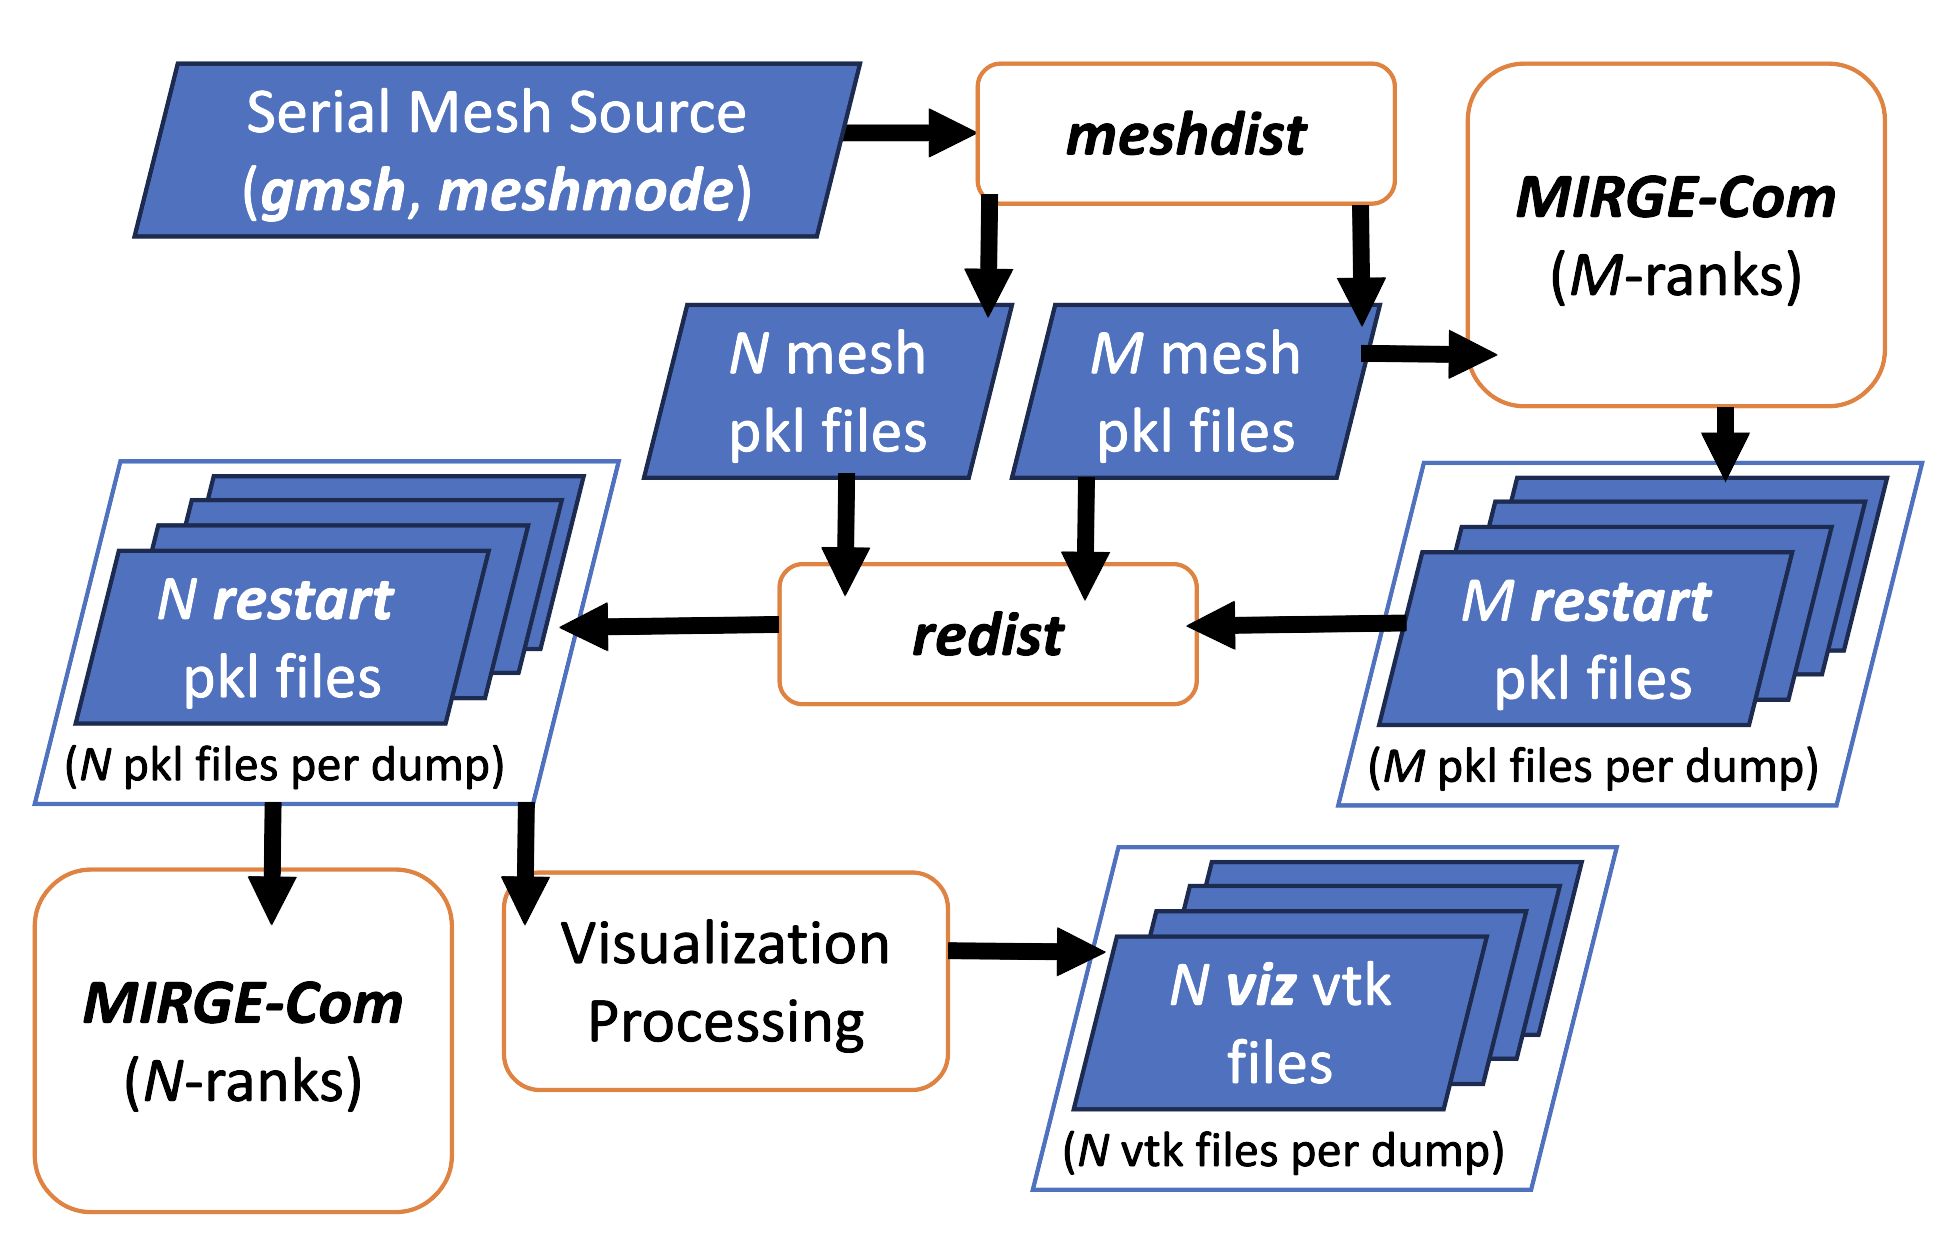
\includegraphics[width=\textwidth]{Figures/mtc/redist_data_flow_full.png}
\end{minipage}
\end{frame}

\begin{frame}\frametitle{TODOs For M-to-N}
  \begin{itemize}
  \item Everything is in \mirgecom{} PR 973 (WIP)
  \item Some things are prediction-specific (gmsh mesh source)
  \item Unkludge the restart debonk (some sort of standardization):
    \begin{itemize}
    \item Auto-detection of DOFArrays in restart data is OK - could be better
    \item Finding partition with all volumes, ugh
    \item Need some way to associate DOFArrays $\rightarrow$ Volume/dd
    \end{itemize}
  \item \textit{Meshmode} support for m-to-n mappings would be nice 
  \end{itemize}
\end{frame}
